\chapter{计算预算有限时的近似优化}
\label{chap:approximate-optimization}

更新公式可以写成一条，执行它却要读取数据、求解子问题并重复多轮。当这些成本超过预算，就必须说明在哪一环让步、引入的误差如何受控。本章固定原问题与预算口径，按被改变的计算对象组织：14.1放宽候选可行集并恢复原解，14.2用主化代理替换当步目标，14.3限制每轮更新的变量范围，14.4改变方向的读取、聚合与反向规则。四种简化不互斥，可以组合；但每种简化只直接控制被简化后的问题，返回候选仍须按原问题的可行性与误差标准核验。

\section{松弛域的构造与原解恢复}

\subsection{精确凸包的基准与恢复问题}

离散选择中变量只能取$0$或$1$，孤立点上没有斜率，无法沿梯度移动；一种做法是把候选放进包含它们的连续凸集，这类放宽称为\term{凸松弛}，可先求较易问题的界，再恢复原解。对非空有限集$S=\{\bm s_1,\ldots,\bm s_N\}$，其凸包
\[
 \operatorname{conv}(S)
 =\left\{\sum_{i=1}^N\alpha_i\bm s_i:
 \alpha_i\geq0,\ \sum_i\alpha_i=1\right\}
\]
是包含$S$的最小凸集；凸包的基本性质已在凸性讨论中建立。若原目标只在$S$上定义，还须选定在$S$上与之一致的连续延拓，才能谈松弛问题的目标。

\paragraph{线性值保持。}
对线性目标$\bm c^\top\bm x$，任意凸包点的目标值是原候选值的加权平均，故$\min_{\operatorname{conv}(S)}\bm c^\top\bm x=\min_S\bm c^\top\bm x$，最大化同理；有限集保证极值达到。但数值相等没有规定求解器返回哪个点。凸集的极点是不能写成非平凡平均的点；线性目标的最优面$K^\star=\{\bm x\in K:\bm c^\top\bm x=M\}$在$K=\operatorname{conv}(S)$时正是原最优点的凸包——给次优点正权重会严格拉低平均值。当$S\subseteq\mathbb Z^d$时最优面含整数极点（可在有限个整数最优点中逐坐标取字典序最大者），但这并不保证任意连续输出都是整数点。

三点集$S=\{(0,0),(1,0),(0,1)\}$同时说明两件事：原候选$(1,0)$与分数点$(1/2,1/2)$在线性目标$x_1+x_2$下值都为$1$，最优数值确实能由原候选取得；但$(1/2,1/2)$本身不属于$S$，求解器返回它仍需恢复规则。

\subsection{线性约束的外逼近松弛}

精确凸包的完整不等式描述可能难以获得，只保留局部约束通常得到更大、更易求解的多面体；对最小化它给更松的下界。容量例
\[
 \max_{x_1,x_2\in\{0,1\}}x_1+x_2
 \quad\text{s.t.}\quad 2x_1+2x_2\leq3
\]
的整数最优值为$1$；放宽到$[0,1]^2$后$(3/4,3/4)$可行且值为$3/2$。四舍五入得$(1,1)$违反容量（容量为$4$），向下取整得$(0,0)$虽可行却损失全部收益。松弛值与原最优值之差$3/2-1=1/2$称为\term{整数间隙}（integrality gap）；松弛值、恢复规则可行性与恢复后损失必须分别分析。

图~\ref{fig:opt-hull-relaxation}并列精确凸包与局部松弛。
\begin{figure*}[htbp]
  \centering
  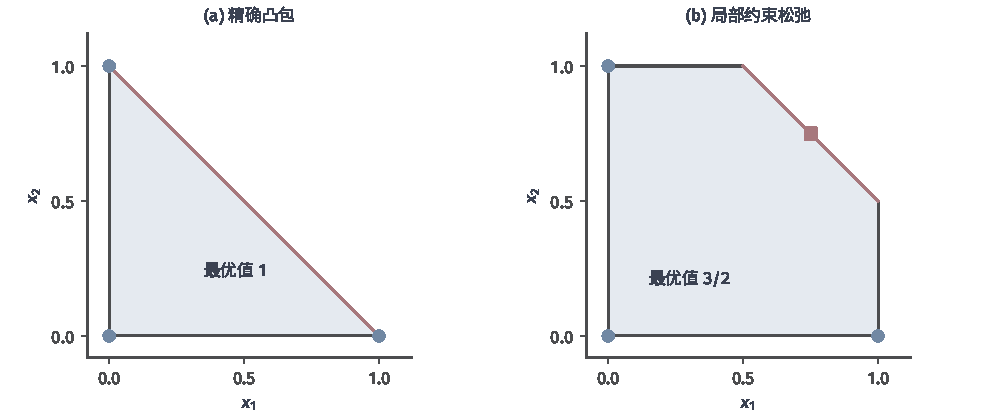
\includegraphics[width=169.0mm]{figures/00-shared/mathematical-preliminaries-upper/04-optimization/matplotlib/opt-hull-relaxation/figure.pdf}
  \caption{最大化$x_1+x_2$的两种放宽。左图精确凸包满足$x_1+x_2\leq1$；右图局部松弛满足$0\leq x_i\leq1$与$x_1+x_2\leq3/2$。实心圆为整数可行点，方形为分数最优点$(3/4,3/4)$，粗边标出最优面。}
 \label{fig:opt-hull-relaxation}
\end{figure*}

\subsection{半正定松弛法}

含乘积$x_ix_j$时引入对称矩阵$\bm X$，精确表示要求$\bm X=\bm x\bm x^\top$（非凸等式），放宽为
\[
 \begin{bmatrix}1&\bm x^\top\\\bm x&\bm X\end{bmatrix}\succeq\bm0
 \quad\Longleftrightarrow\quad \bm X-\bm x\bm x^\top\succeq\bm0,
\]
等价性由$(t+\bm x^\top\bm v)^2+\bm v^\top(\bm X-\bm x\bm x^\top)\bm v$配方核对。真实乘积满足新约束，新约束却允许偏离真实乘积；新增矩阵有$O(d^2)$个元素，需求解锥约束。返回$(\widehat{\bm x},\widehat{\bm X})$后要分别核验原约束与$\widehat{\bm X}=\widehat{\bm x}\widehat{\bm x}^\top$，矩阵提升本身不完成原解恢复。集合函数的连续扩展还须针对所选扩展检验凸凹性，“次模”（离散次模不等式）本身不判定延拓的凸性；二值成对能量的图割表示是后续图章在特定条件下展开的接口。

\section{主化—最小化代理法（MM）}

\subsection{MM的代理构造、接受与误差}

梯度下降的闭式步长来自下降引理给出的可计算二次上界。把这一思想一般化：在当前点构造一个处处不低于原目标、又在当前点贴合的简单函数。

\begin{definition}[主化代理与MM更新]
\label{def:opt-majorization-minimization}
给定目标$F:C\to\mathbb R$与当前点$\bm w^{(t)}\in C$，代理$Q(\bm w\mid\bm w^{(t)})$满足
\[
 F(\bm w)\leq Q(\bm w\mid\bm w^{(t)}),\qquad
 F(\bm w^{(t)})=Q(\bm w^{(t)}\mid\bm w^{(t)})\quad(\forall\bm w\in C).
\]
若新点满足代理值不增$Q(\bm w^{(t+1)}\mid\bm w^{(t)})\leq Q(\bm w^{(t)}\mid\bm w^{(t)})$，称为\term{主化--最小化方法}（majorization--minimization，MM）的改善更新。
\end{definition}

改善链为
\[
 F(\bm w^{(t+1)})
 \leq Q(\bm w^{(t+1)}\mid\bm w^{(t)})
 \leq Q(\bm w^{(t)}\mid\bm w^{(t)})
 =F(\bm w^{(t)}),
\]
三步分别用全局上界、代理改善与切触；上界只在局部有效时，新点越界就断链。$L$光滑目标的下降引理二次型就是代理：全空间精确最小化给$1/L$梯度步，闭凸集上给投影梯度。不精确最小化时，记代理最优值$Q^{\star,(t)}$与改善空间$\Delta^{(t)}=Q(\bm w^{(t)}\mid\cdot)-Q^{\star,(t)}$，若
\[
 Q(\bm w^{(t+1)}\mid\bm w^{(t)})\leq Q^{\star,(t)}+\epsilon^{(t)},
\]
则$F(\bm w^{(t+1)})\leq F(\bm w^{(t)})-\Delta^{(t)}+\epsilon^{(t)}$；只有$\epsilon^{(t)}\leq\Delta^{(t)}$才保证本轮不增。原目标有有限下界时$\sum_{t<T}\Delta^{(t)}\leq F(\bm w^{(0)})-\inf_CF+\sum_t\epsilon^{(t)}$。数值例$F(x)=x^2/2$、$Q(x\mid1)=(x-1/2)^2+1/4$中，求到$x=3/4$仍改善（$9/32<1/2$），返回$x=5/4$时代理误差$9/16$超过改善量$1/4$，原目标反升为$25/32$。

图~\ref{fig:opt-majorizer-versus-tangent}对照代理上界与同斜率切线。
\begin{figure}[htbp]
  \centering
  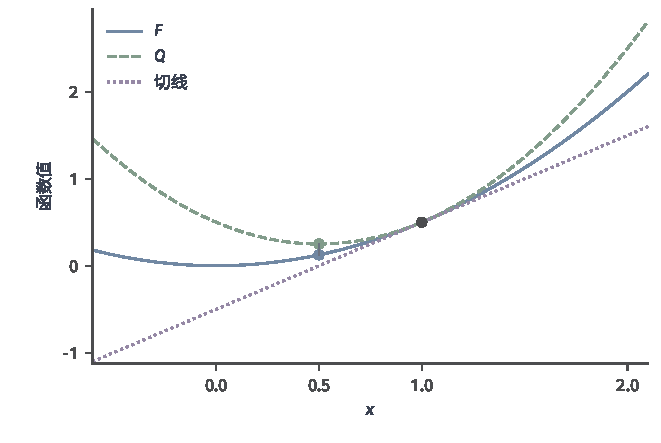
\includegraphics[width=112.0mm]{figures/00-shared/mathematical-preliminaries-upper/04-optimization/matplotlib/opt-majorizer-versus-tangent/figure.pdf}
  \caption{代理上界与切线的区别。蓝线$F(x)=x^2/2$，绿虚线为当前点$1$处的主化代理，紫点线为同点切线$x-1/2$。三者在当前点同值同斜率，但切线位于目标下方，不能使用MM的上界链。}
 \label{fig:opt-majorizer-versus-tangent}
\end{figure}

\subsection{MM的残差实现：IRLS}

平方代价使残差$10$的贡献是残差$1$的百倍。保持残差定义不变，改用增长较慢的代价$F(\bm w)=\frac12\sum_i\rho(r_i(\bm w)^2)$：平方损失$\rho(s)=s$；尺度$c>0$下Cauchy代价$c^2\log(1+s/c^2)$；Tukey代价在$s\leq c^2$时为$c^2[1-(1-s/c^2)^3]/3$、其后恒为$c^2/3$。单项对残差的斜率分别为$r$、$r/(1+r^2/c^2)$和$r(1-r^2/c^2)^2\mathbb I\{|r|\leq c\}$，大残差处边际代价减弱；参数梯度还乘$\nabla r_i$，且代价非凸，初始化与尺度影响驻点。

若$\rho$可微、非减且关于$s$凹，凹函数在切线下，故$\rho(s)\leq\rho(s_0)+\rho'(s_0)(s-s_0)$。在当前残差$s_i^{(t)}=r_i(\bm w^{(t)})^2$处构造代理
\begin{equation}
 Q(\bm w\mid\bm w^{(t)})
 =\mathrm{const}^{(t)}
 +\frac12\sum_i a_i^{(t)}r_i(\bm w)^2,
 \qquad a_i^{(t)}=\rho'(s_i^{(t)})\geq0,
 \label{eq:opt-irls-majorizer}
\end{equation}
每轮“算权重—固定权重解加权最小二乘—重算残差权重”，即\term{迭代重加权最小二乘}（iteratively reweighted least squares，IRLS）。Cauchy权重为$(1+s_i/c^2)^{-1}$，Tukey权重为$(1-s_i/c^2)^2\mathbb I\{s_i\leq c^2\}$；权重来自同一目标的切线，不能任意重设。线性残差时子问题是加权最小二乘（权重平方根各行相乘后用QR/SVD），非线性残差时可在内部调用Gauss--Newton或LM，但一次线性化方程解不保证完整代理下降，必须核验代理值。用常数$w$拟合$0,0,10$，Cauchy（$c=1$，$w^{(0)}=0$）首轮权重$1,1,1/101$给$w^{(1)}=10/203$；Tukey可能让全部权重为零、代理退化为常数，此时应检查初始化或尺度。永久正则项须原样进入每轮代理，不能与内部控制位移的阻尼混同。

\section{块坐标更新}

本节把一次全变量更新拆成若干小问题，这类按变量块更新的路线称为\term{分块坐标法}。

\subsection{块梯度与块邻近更新}

变量自然分成$\bm u\in\mathbb R^p$、$\bm v\in\mathbb R^q$时，对
\[
 \Phi(\bm u,\bm v)=\frac12\|\bm X\bm u+\bm Z\bm v-\bm y\|_2^2+r(\bm u)+s(\bm v)
\]
可固定其余块，只对当前块作梯度或邻近一步，每完成一块就用同一$\Phi$核验改善。固定$\bm v$时光滑项对$\bm u$的光滑常数为$\|\bm X\|_2^2$，邻近步长取$0<\eta_u\leq1/\|\bm X\|_2^2$；近似输出仍须实际接受条件。

\subsection{块条件最小化：交替最小化}

\term{交替最小化}依次精确或近似求解固定其他块后的条件子问题：
\[
 \Phi(\bm u^{(t+1)},\bm v^{(t)})\leq\Phi(\bm u^{(t)},\bm v^{(t)}),\qquad
 \Phi(\bm u^{(t+1)},\bm v^{(t+1)})\leq\Phi(\bm u^{(t+1)},\bm v^{(t)}),
\]
两条不等式串成同一轮下降，多解时要规定平局选解规则。耦合正定二次例$\Phi(u,v)=\frac12(u-v)^2+\frac12(u-1)^2$给$v^{(t+1)}-1=(v^{(t)}-1)/2$，收敛到$(1,1)$；但$(uv-1)^2$从$(0,0)$出发时，任一块固定为零目标都是常数，平局规则选零就停在目标$1$，而全局最优为$0$——逐块精确、分别凸都不保证全局最优。无约束连续可微时，每块最优给各偏导为零，合起来是联合驻点；联合凸时才足以给全局最优，且还要证明实际迭代到达块最优点。

有限分布变量就是概率单纯形$\bm\Delta_m=\{\bm q:q_i\geq0,\sum_iq_i=1\}$上的向量，块更新后必须留在单纯形内。把$\bm q$投影到$\bm\Delta_2$、目标中心$(0.8,0.4)^\top$的解为$(0.7,0.3)^\top$（共减阈值$0.1$），它真实最小化当前条件目标。EM与变分方法在期望与散度对象建立后复用这里的交替优化与MM核验。副本协调式的对偶分解（改进对偶下界、原目标不逐轮下降）与本节同一原目标上的交替改善是两条路线，不能互相代替。

\section{方向的读取、聚合与变换}

有限和目标
\[
 F_S(\bm w)=\frac1n\sum_{i=1}^n\ell_i(\bm w)+\frac{\lambda}{2}\|\bm w\|_2^2
\]
的完整梯度要读取全部$n$项。以下只用有限概率权重的加权平均（记固定历史后的平均为$\mathbb E^{(t)}$）；长期随机收敛与泛化留到概率工具。

\subsection{索引分布与重加权}

均匀抽取$I$时，$\bm g_I(\bm w)=\nabla\ell_I(\bm w)+\lambda\bm w$的固定历史平均等于$\nabla F_S$；非均匀概率$p_i>0$时须按$1/(np_I)$反比重加权：
\[
 \bm g_I(\bm w)=\frac{\nabla\ell_I(\bm w)}{np_I}+\lambda\bm w.
\]
正则梯度是确定量，不抽样也只加一次。标量梯度$2,-1$以$3/4,1/4$直接平均得$5/4$，重加权读数$4/3,-2$才恢复均值$1/2$；小权重会放大读数，无偏不意味波动更小。

\paragraph{样本替换的有限步响应。}
固定两个只差一个样本的数据集$S,S'$、共同初值、相同索引路径与步长。设每样本梯度$L$-Lipschitz、访问点范数不超过$G$，命中替换项时距离增量至多$2\eta G$；若每样本损失凸且$0\leq\eta\leq2/L$，单样本更新非扩张，去掉膨胀因子，固定历史平均给期望参数距离
\begin{equation}
 \mathbb E\,\Delta^{(T)}\leq\frac{2G}{n}\sum_{t<T}\eta^{(t)}.
 \label{eq:opt-stability-distance}
\end{equation}
经验目标凸不替代逐样本凸；测试损失为$K$-Lipschitz时损失差再乘$K$。这是耦合相同随机索引下的\term{算法稳定性}界，需条件期望工具才能作严格随机表述，也不直接是泛化定理。沿途梯度界可在非负光滑损失上自举：$\ell\geq0$且$L$光滑时，下降引理取$\bm v=\bm w-\nabla\ell/L$给
\begin{equation}
 \|\nabla\ell(\bm w)\|_2^2\leq2L\ell(\bm w),
 \label{eq:opt-self-bounding}
\end{equation}
但只在损失值已有上界的点上有效，不是全局梯度界。

\subsection{批量聚合与梯度累积}

固定历史后，$b$个独立无偏、均方波动不超过$(\sigma^{(t)})^2$的读数平均，交叉项均值为零，均方波动降至$(\sigma^{(t)})^2/b$；重复同一样本无此收益，增大批量也不消除系统偏差$\bm b^{(t)}$。有偏读数可写成$\bm g^{(t)}=\nabla F_S+\bm b^{(t)}+\bm\xi^{(t)}$，批量只压低$\bm\xi$。

微批量累积把同一次更新的读数分成$K$组，在冻结的参数$\bm w$处算$n_j^{-1}\sum_{i\in B_j}\nabla\ell_i$，按样本数加权累计$N^{-1}\sum_jn_j\bm g_j$，只加一次$\lambda\bm w$，整个窗口不推进动量、Adam统计和调度时钟。$n_1=2,n_2=1$、组均值$1,4$时总均值为$2$而非$5/2$；等价还要求各项实际函数、随机状态与求值点相同，BatchNorm或Dropout等批内相互作用会改变结果。累积是$K$次读取加一次参数更新，不是零成本的一次大批量。

\subsection{已有读数的梯度裁剪}

逐元素裁剪$[\operatorname{clip}^{\rm elem}_c(\bm g)]_k=\max(-c,\min(c,g_k))$限制各坐标；整体范数裁剪$\operatorname{clip}_c(\bm g)=\bm g\min\{1,c/\|\bm g\|\}$保持方向、限制范数。$\bm g=(3,4)^\top$、$c=1$下前者给$(1,1)^\top$（范数$\sqrt2$、方向改变），后者给$(3/5,4/5)^\top$。裁剪改变读数平均，等概率$2,-1$截到$1$后均值由$1/2$变$0$，增大批量不会自动恢复；裁剪发生在历史统计之前还是之后、裁读数还是裁最终位移，是不同算法，须把实际方向与参考梯度之差计入误差。

\subsection{离散前向的替代梯度与STE}

阈值、取整运算在大部分位置局部常数，真实导数为零。\term{替代梯度}是人为指定的反向信号，既不是经典导数也通常不满足次梯度不等式；中心差分核验的是实际前向函数，不能要求它等于指定反向。令$Q(w)=\operatorname{round}(w)$、$F(w)=\ell(Q(w))$，\term{直通估计}（straight-through estimator，STE）把$Q$的反向导数指定为$1$，返回$g_{\rm STE}(w)=\ell'(Q(w))$。$\ell(z)=(z-a)^2/2$：$w=0.2,a=1$时真实导数为零、STE给$-1$，步长$0.4$跨阈值后损失降为零；同一$w$、$a=0.4$、步长$1$把点推到$0.6$，损失却由$0.08$升到$0.18$，不能套用光滑下降证明。向量量化前向选最近码向量$\bm e_{k^\star}$，反向用计算图标记$\bm z=\bm x+\operatorname{sg}(\bm e_{k^\star}-\bm x)$指定单位Jacobian；$\operatorname{sg}$是停止传播标记，不是“恒等取值且经典导数为零”的普通函数，码向量更新还要另行规定。

\section{原问题的输出质量、收敛与预算评价}

\paragraph{可行输出与目标差证书。}
返回结果首先说明属于原可行域还是松弛域。对最小化问题，原可行候选给上界$U$，精确松弛值、合法对偶值或带可信误差修正的下界给$L$，$0\leq U-p^\star\leq U-L$；松弛候选值本身不能当$L$，恢复点要单独算$f(\widehat{\bm x})-L$。

\paragraph{改善、驻点与参数收敛。}
MM链与同目标分块更新控制原目标值，松弛值描述另一候选域，均方读数误差描述方向信息，三者分别报告。目标逐轮不增且有有限下界只推出目标值有极限；参数收敛、聚点驻点与全局最优是进一步问题，权重退化与$(uv-1)^2$平局停滞分别给出缺口。

\paragraph{尺度一致性与总预算。}
损失乘常数$a>0$会把梯度与光滑常数同乘$a$，比较学习率前先固定损失归一化口径。预算比较先固定输出（可行点与证书、驻点残差或有限步轨迹），再合计外层轮数、样本读取、试探求值、子问题求解、锥求解与可行恢复成本；矩阵提升的$O(d^2)$存储、微批量的读取／更新次数区别、调度求值都要计入，减少外层次数不自动减少总计算。

\section{本章小结}

四类让步各改一个对象：松弛换候选集合，MM换当步函数，分块限制变量，近似更新改变方向信息。子问题误差分别进入代理改善量（$\epsilon^{(t)}$对$\Delta^{(t)}$）或可信对偶界（减去$\epsilon$）。LM在原残差目标上控制位移并用真实下降接受，IRLS由同一残差代价的切线上界重分配权重，STE另定离散反向：前两者在相应条件下核验下降，STE必须直接检查前向损失。光滑下降的加权平方误差、轨迹偏差的一次范数误差、副本一致性残差控制不同对象，不合成单一精度数。下一章改变的是问题定义本身：多个指标的取舍、对立两方的响应次序与内层选解。
